% Capítulo 12: herança, com Forma abstrata e as classes Retangulo e Circulo.
\documentclass[border=4pt]{standalone}
\usepackage[utf8]{inputenc}
\usepackage[T1]{fontenc}
% Estilo comum dos fluxogramas e diagramas de blocos.
\usepackage{tikz}
\usetikzlibrary{arrows.meta, positioning, calc, shapes.geometric, shapes.misc}
\definecolor{navy}{RGB}{23,45,80}
\definecolor{laranja}{RGB}{250,110,29}
\definecolor{cinzalogo}{RGB}{107,114,126}
\definecolor{azul}{RGB}{205,222,247}
\tikzset{
  base/.style={draw=navy, line width=0.9pt, font=\sffamily\small, align=center, inner sep=4pt},
  terminal/.style={base, rounded rectangle, fill=laranja!45, draw=laranja, minimum width=20mm, minimum height=7mm},
  processo/.style={base, rectangle, fill=laranja!12, minimum width=28mm, minimum height=8mm},
  decisao/.style={base, diamond, aspect=2.2, fill=azul, inner sep=1pt, minimum width=30mm},
  es/.style={base, trapezium, trapezium left angle=72, trapezium right angle=108,
             fill=white, minimum width=26mm, minimum height=8mm, trapezium stretches body},
  fluxo/.style={-{Stealth[length=2.2mm]}, navy, line width=0.9pt},
  rotulo/.style={font=\sffamily\small\bfseries, text=navy},
  legenda/.style={font=\sffamily\scriptsize, text=cinzalogo},
  resposta/.style={font=\sffamily\scriptsize\bfseries, text=navy},
}

\usetikzlibrary{shapes.multipart}
\tikzset{
  classe/.style={rectangle split, rectangle split parts=3, draw=navy, line width=0.9pt,
                 rectangle split part fill={laranja!45, laranja!12, laranja!12},
                 font=\ttfamily\scriptsize, align=left, inner sep=4pt, text width=34mm},
  abstrata/.style={classe, rectangle split part fill={azul, azul!40, azul!40}},
  herda/.style={-{Triangle[open, length=3mm, width=3mm]}, navy, line width=0.9pt},
}
\begin{document}
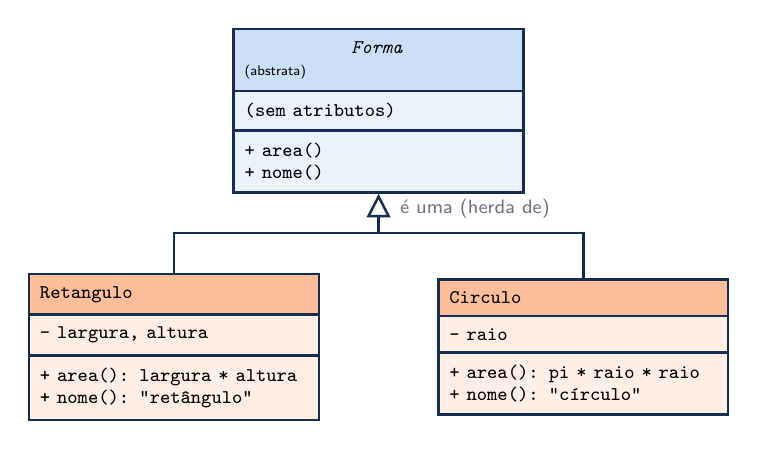
\begin{tikzpicture}
  \node[abstrata] (f) at (0, 0) {\centering\textbf{\textit{Forma}}\\{\sffamily\tiny (abstrata)}
    \nodepart{two} (sem atributos)
    \nodepart{three} + area()\\+ nome()};
  \node[classe] (r) at (-2.6, -3.0) {\centering\textbf{Retangulo}
    \nodepart{two} - largura, altura
    \nodepart{three} + area(): largura * altura\\+ nome(): "retângulo"};
  \node[classe] (c) at (2.6, -3.0) {\centering\textbf{Circulo}
    \nodepart{two} - raio
    \nodepart{three} + area(): pi * raio * raio\\+ nome(): "círculo"};
  \coordinate (m) at (0, -1.55);
  \draw[navy, line width=0.9pt] (r.north) |- (m) -| (c.north);
  \draw[herda] (m) -- (f.south);
  \node[legenda, anchor=west] at (0.15, -1.25) {é uma (herda de)};
\end{tikzpicture}
\end{document}
